\documentclass[12pt]{article}
\usepackage[margin=1in]{geometry}
\usepackage{graphicx}
\usepackage{subcaption}

\begin{document}
\title{StyleGAN and StyleGAN2 for Face Morphing Applications}
\author{Jason Kuo}
\date{March 2021}
\maketitle

\begin{abstract}
\end{abstract}

\section{Introduction}
\par
Face recognition is an important feature in many systems today, including unlocking personal devices and verifying identity. One particular application of note is an eGate system which is used to automatically permit authenticated users into a restricted area such as for boarding a plane \cite{magic-passport}. Face recognition, along with other biometric verification systems, are used by comparing the known data about an individual (such as their face on a passport image) to new data at the gate (for example, by taking a live picture with a webcam).
\par
Face morphing poses a potential security threat to systems like these because if a morph is successfully submitted as a passport photo, it could authenticate multiple users with the same image \cite{magic-passport}. There are several methods for generating these morphs. Traditionally, landmark-based morphing methods have been used to detect important facial landmarks and interpolate between the corresponding landmarks for each face contributing to the morph (usually only 2). The best versions of these methods require manual placement of landmarks, which is extraordinarily slow and labor intensive. This process can be automated, but many of the current fully automatic landmark-based algorithms produce easily seen morphing artifacts.
\par
A more modern approach is to use Generative Adversarial Networks (GANs) to produce morphs. In general, GANs attempt to generate new data from the underlying distribution of input data \cite{goodfellow2014generative}. They do this by constructing two neural networks, a generator and a discriminator, and setting them against each other in a zero-sum game. The generator's goal is to learn to generate data samples similar to the input data for the purpose of fooling the discriminator, whereas the discriminator's goal is to learn to distinguish which samples come from the actual input and which come from the generator. After training, the generator with its learned model should be able to produce data similar to the input, but not exactly copying the input. For the specific example of face images, GANs usually train two convolutional neural networks. Most GANs produce the output image starting with some latent vector representation, meaning that we can think of a GAN as mapping an input vector to a face image and training the GAN as defining that mapping. For a given input face, if we can find the representation such that the output after GAN processing is as close to the input face as possible, then we can simply interpolate between two such representations to generate morphs between the two faces that those vectors represent. Interpolation is meaningful \cite{abdal2019iamge2stylegan} in the context of GANs because they attempt to learn a smooth mapping from the latent space of representations to the output images.
\par
In this paper, we will try to evaluate some GAN-based morphing methods and compare them with a landmark-based method. We will primarily focus on modifying and using StyleGAN and StyleGAN2 to generate these GAN-based morphs.

\begin{figure}
    \centering
    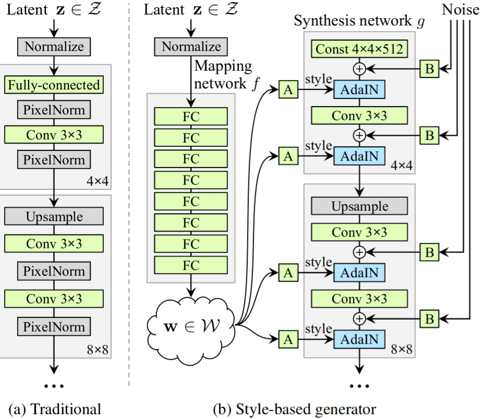
\includegraphics{sgan1_arch.png}
    \caption{The style-based architecture of StyleGAN maps a latent vector $\mathbf{z}$ to an intermediate latent vector $\mathbf{w}$ whereas a traditional generator only feeds the latent vector into the input layer. StyleGAN then feeds the intermediate $\mathbf{w}$ into different layers for each resolution to produce a high resolution result.}
    \label{sgan1_arch}
\end{figure}
\section{StyleGAN}
\par
StyleGAN \cite{stylegan} is a GAN architecture (Figure \ref{sgan1_arch}) from NVIDIA which is able to generate high quality and high resolution images. It is inspired by style transfer literature which emphasizes the importance of meaningful interpolation properties. Thus, it is very useful for morphing applications. By default, as well as in our pipeline, StyleGAN is trained on the FFHQ dataset consisting of 70,000 high-quality face images at 1024x1024 resolution collected from Flickr. However, one problem with the original StyleGAN is that it does not provide a means for finding the latent vector that corresponds to a given input image. That is, the inverse mapping that converts from a face image to a latent vector is not learned with NVIDIA's implementation.

\par
% StyleGAN-encoder
A popular implementation that does provide this functionality is the stylegan-encoder repository \cite{stylegan-encoder}. It uses a pre-trained VGG16 network to calculate the feature vectors for the given input image and an initial StyleGAN generated image. A loss function is defined as the difference between these two vectors. Then, it minimizes this loss by changing the generated image to obtain the encoded latent representation for the input image.

\section{StyleGAN2}
\par
More recently, NVIDIA released an improved version of StyleGAN named StyleGAN2 \cite{stylegan2}. It builds on the original by focusing on removing normalization artifacts which take the form of blurry blobs in the image. It also improves the image quality and provides built in projection functionality for mapping from an image to its latent representation. Their projector mainly differs from the third-party stylegan-encoder by focusing on finding latent representations that the StyleGAN2 generator could have produced. In constrast, the details of the stylegan-encoder's methodology ends up extending the latent space, which allows encoding arbitrary images that would not otherwise have a latent representation. This crucial difference propagates to our morph results as we will see.

\section{Experimental Methods}
\par
Our goal is to evaluate to what extent a face recognition algorithm is fooled by GAN-generated morphs. To this end, we set up a pipeline for generating morphs, feeding them into a face recognition algorithm, and analyzing the recognition scores produced.

\begin{figure}[t]
    \centering
    \begin{subfigure}{0.19\textwidth}
        \centering
        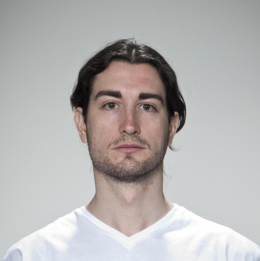
\includegraphics[width=\textwidth]{morph_example_A.png}
        \caption{Subject A}
        \label{morph_comp_1}
    \end{subfigure}
    \begin{subfigure}{0.19\textwidth}
        \centering
        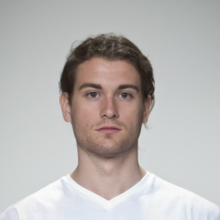
\includegraphics[width=\textwidth]{landmark_morph.png}
        \caption{Landmark morph}
        \label{morph_comp_2}
    \end{subfigure}
    \begin{subfigure}{0.19\textwidth}
        \centering
        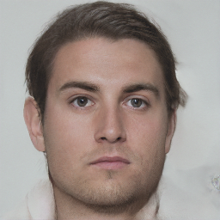
\includegraphics[width=\textwidth]{sgan1_morph.png}
        \caption{stylegan-encoder morph}
        \label{morph_comp_3}
    \end{subfigure}
    \begin{subfigure}{0.19\textwidth}
        \centering
        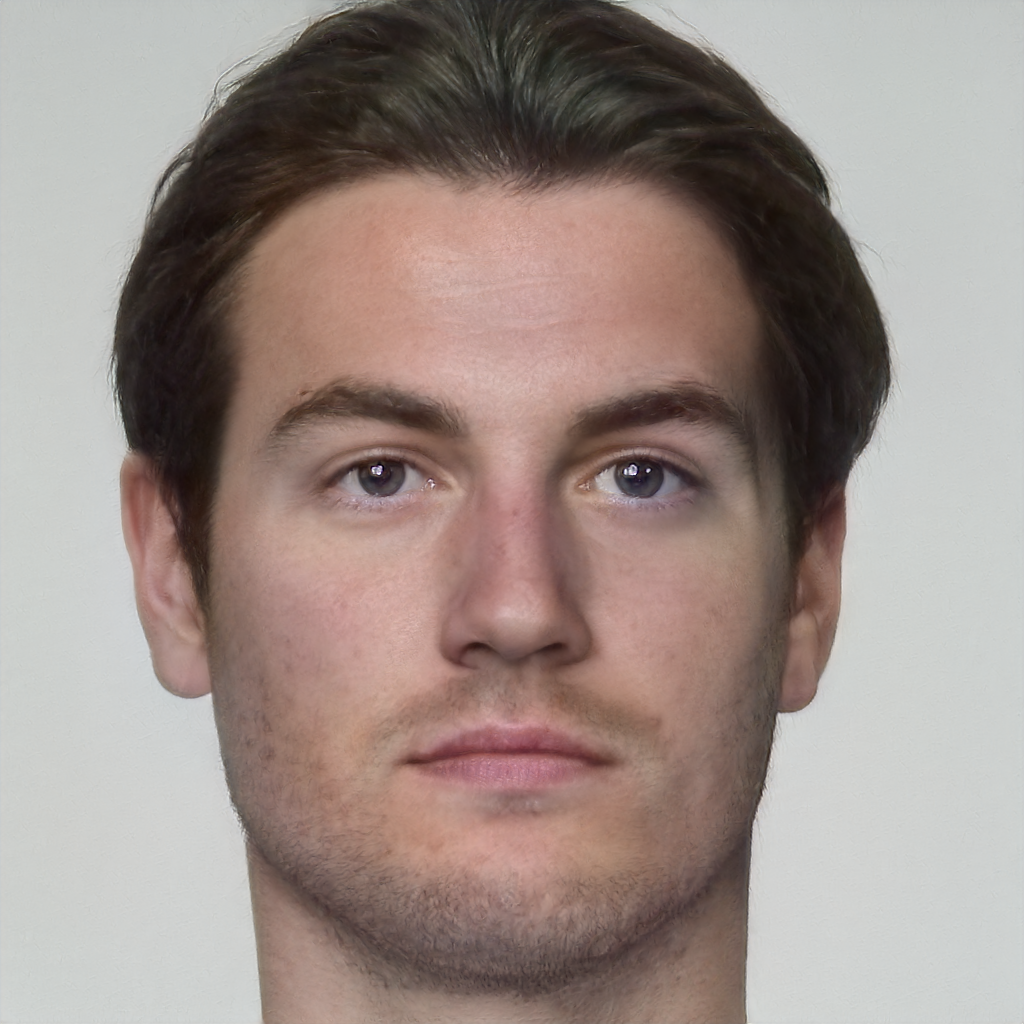
\includegraphics[width=\textwidth]{sgan2_morph.png}
        \caption{StyleGAN2 morph}
        \label{morph_comp_4}
    \end{subfigure}
    \begin{subfigure}{0.19\textwidth}
        \centering
        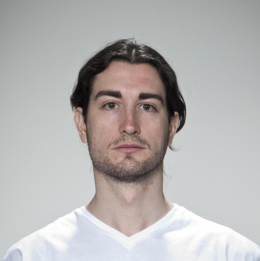
\includegraphics[width=\textwidth]{morph_example_A.png}
        \caption{Subject B}
        \label{morph_comp_5}
    \end{subfigure}

\subsection{Setup}
\par
We implemented this pipeline on a CentOS 7.6 machine with 2 Intel Xeon CPUs and 2 Tesla K40m NVIDIA GPUs. We tested using the Face Research Lab London Dataset \cite{london}. This dataset was separated into male and female faces so that morphs would only be generated within gender. Then, using both the stylegan-encoder and the StyleGAN 2 projector, 50-50 morphs (equal contribution morphs generated using 0.5 as the interpolation coefficients) were generated between each pair of faces within each gender group.
\par
These morphs were evaluated using the \texttt{face\_recognition} Python module which is a wrapper around Dlib's face recognition features. This module produces a face distance $d$ which is then inverted with $1-d$ to produce a similarity score for our evaluation. We compared each morph with the two images from which it is generated to produce the morph distribution. We also generate a genuine distribution by comparing between the neutral and smiling versions of each face and an impostor distribution by comparing between neutral images of different people.
\par
As another baseline, we also generated landmark-based morphs by automatically detecting important landmarks of the faces, averaging them, and splicing them onto one of the initial faces as described by \cite{visapp17}. During evaluation, these landmark morphs are also compared with each of the two images that went into it.

\begin{figure}[t]
    \centering
    \begin{subfigure}{0.45\textwidth}
        \centering
        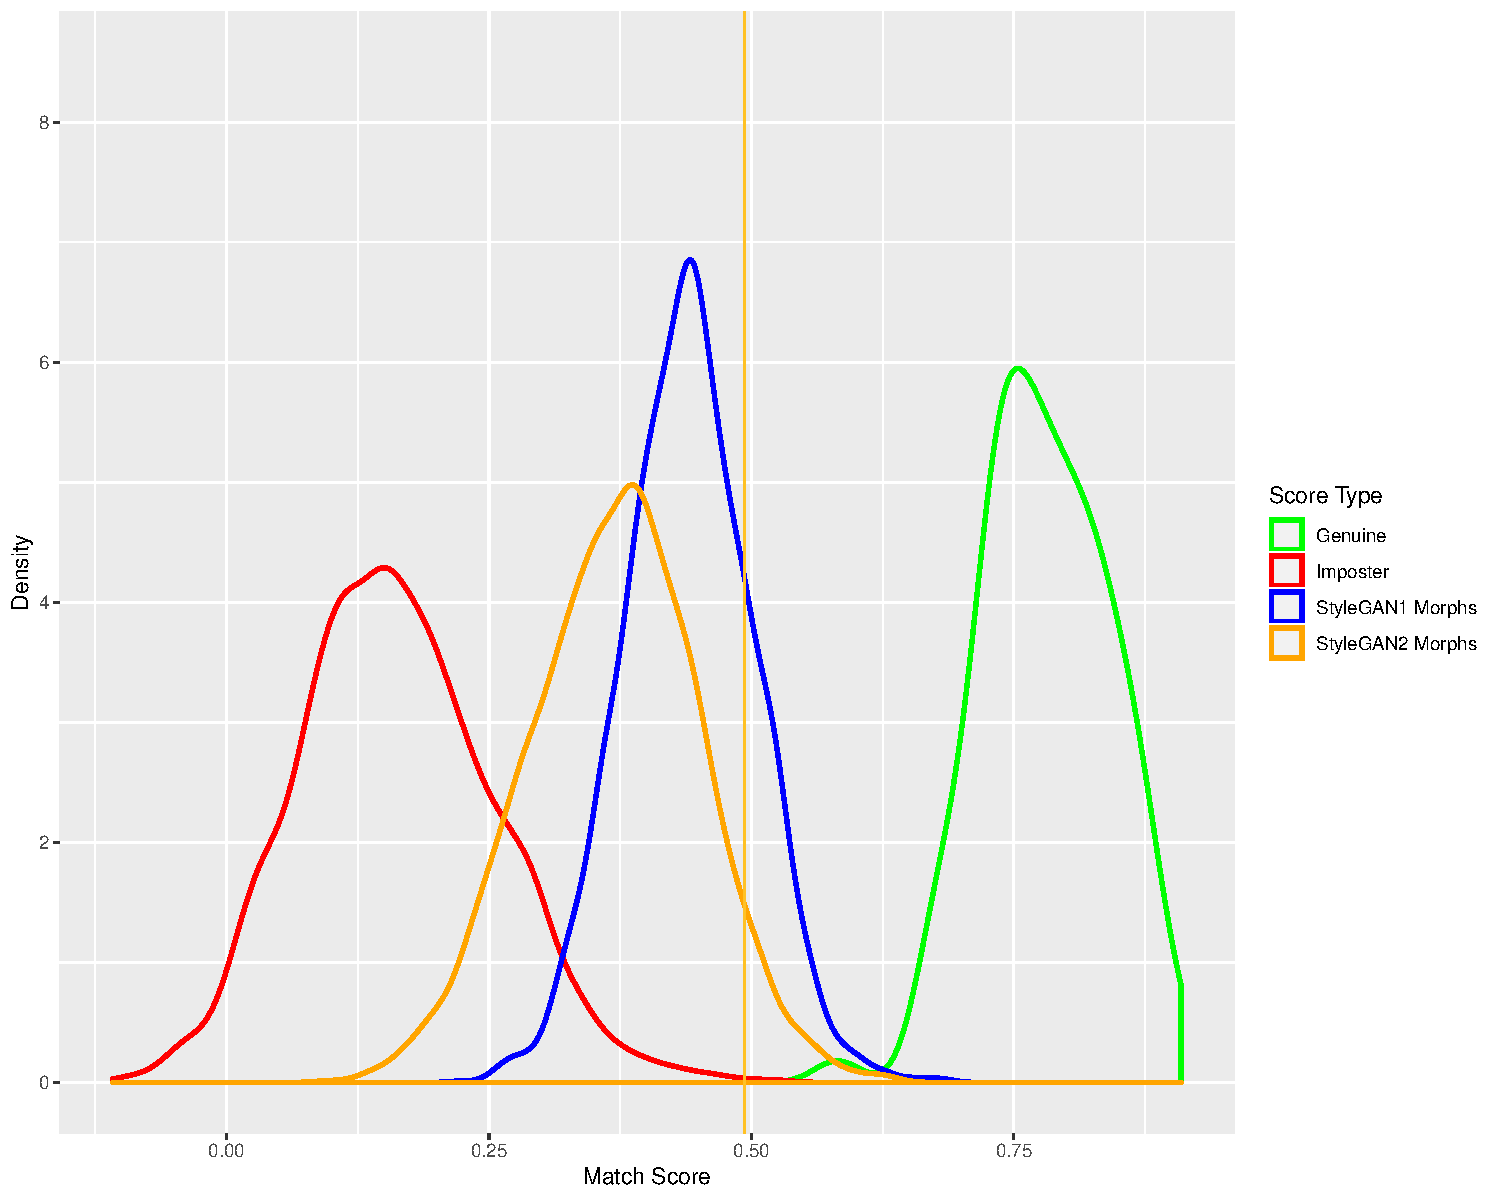
\includegraphics[width=\textwidth]{dlib_fr_gan_hist.pdf}
        \caption{Plot of morph score distributions}
        \label{gan_plot}
    \end{subfigure}
    \begin{subfigure}{0.45\textwidth}
        \centering
        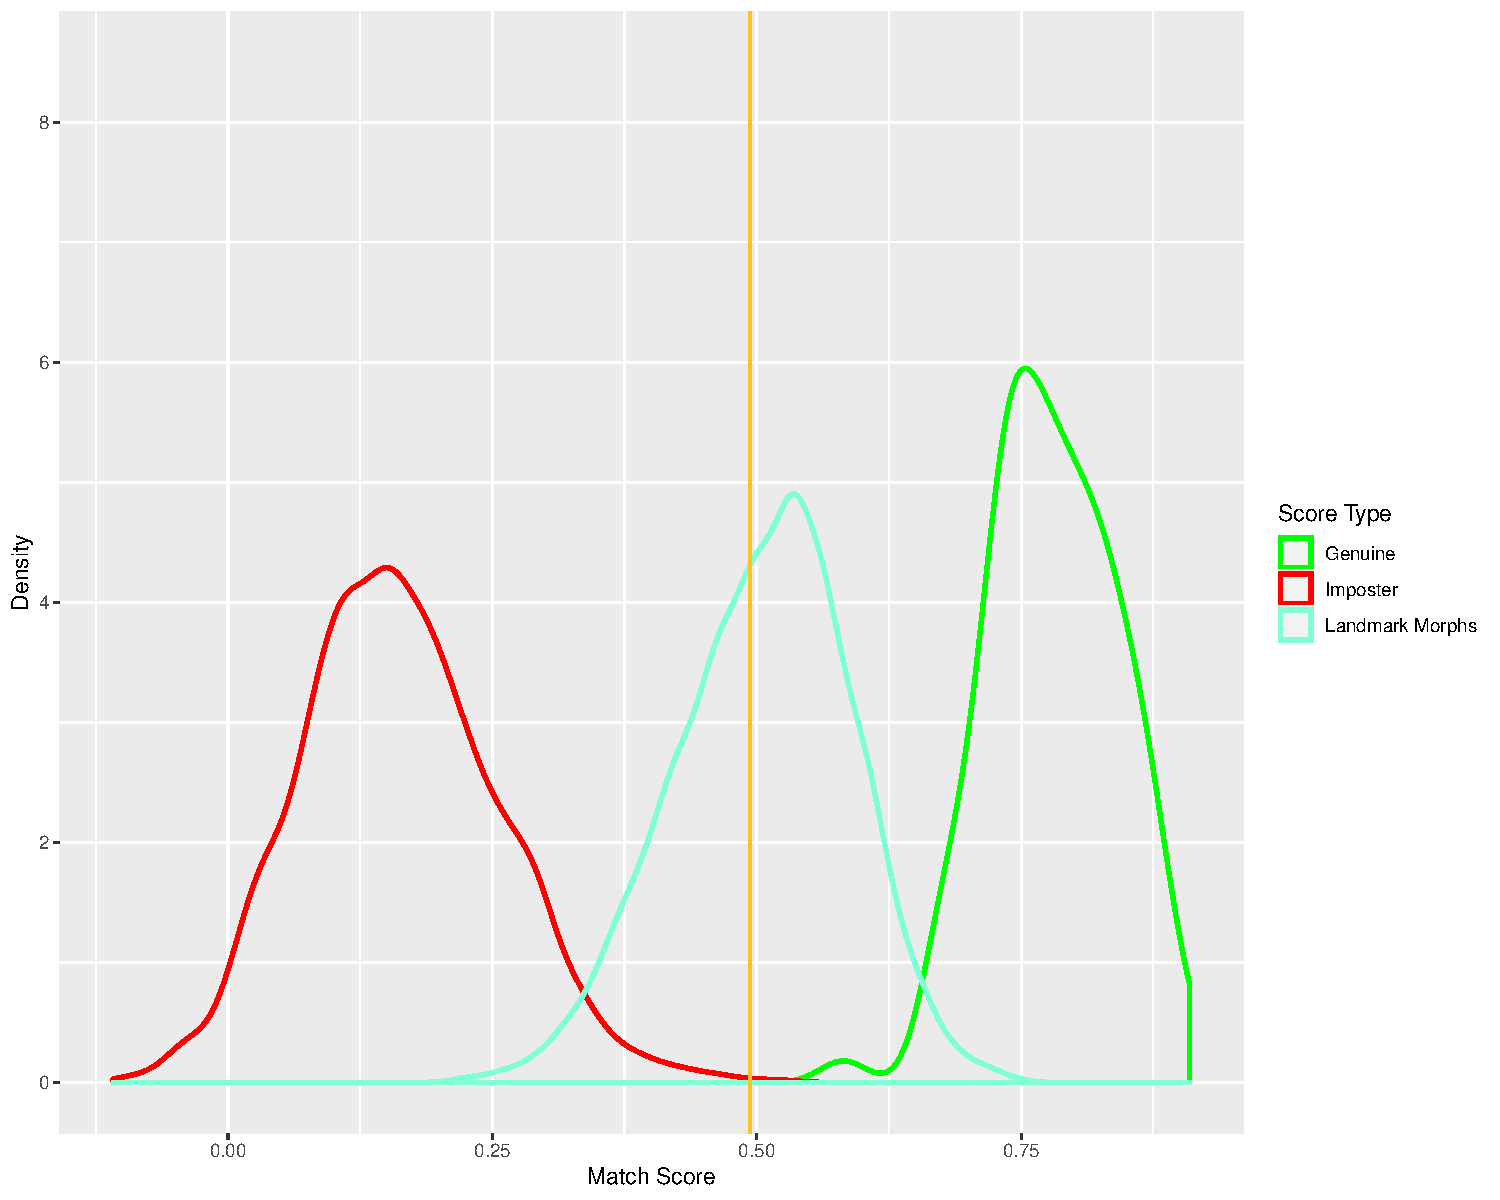
\includegraphics[width=\textwidth]{dlib_fr_landmark_hist.pdf}
        \caption{Plot of landmark morph scores}
        \label{landmark_plot}
    \end{subfigure}
    \caption{The vertical golden line indicates the score threshold for 0.1\% false match rate, meaning that only 0.1\% of impostors would trick this algorithm if it used this score threshold for classification.}
\end{figure}
\subsection{Results}
\par % Citation about 0.1 FMR?, Find proportion of distribution about threshold
Figure \ref{gan_plot} shows the score distributions for the GAN-based morphs generated using the Dlib-based face recognition algorithm. The vertical line represents an important threshold because 0.1\% false match rate (FMR) is a common metric used to calibrate face recognition systems. Since FMR is only calculated based on our invariant impostor distribution, this threshold will be constant at a score of 0.494 for the rest of our analyses. The median score for the stylegan-encoder morphs is 0.440 whereas the median score for the StyleGAN2 projector is 0.372. Similarly, figure \ref{landmark_plot} shows the score distribution for our landmark based algorithm. The median landmark morph score is higher at 0.512.
\par
The proportion of the stylegan-encoder morphs that are above the threshold was 0.192. For the StyleGAN2 projector that becomes 0.059. For the landmark morphs, it is 0.580.
\par
Learning the latent vectors through the stylegan-encoder took about 6 minutes per face whereas doing the same with the StyleGAN2 projector took about 20 minutes per face. After this process, generating morphs took only a couple seconds per morph.

\begin{figure}[t]
    \centering
    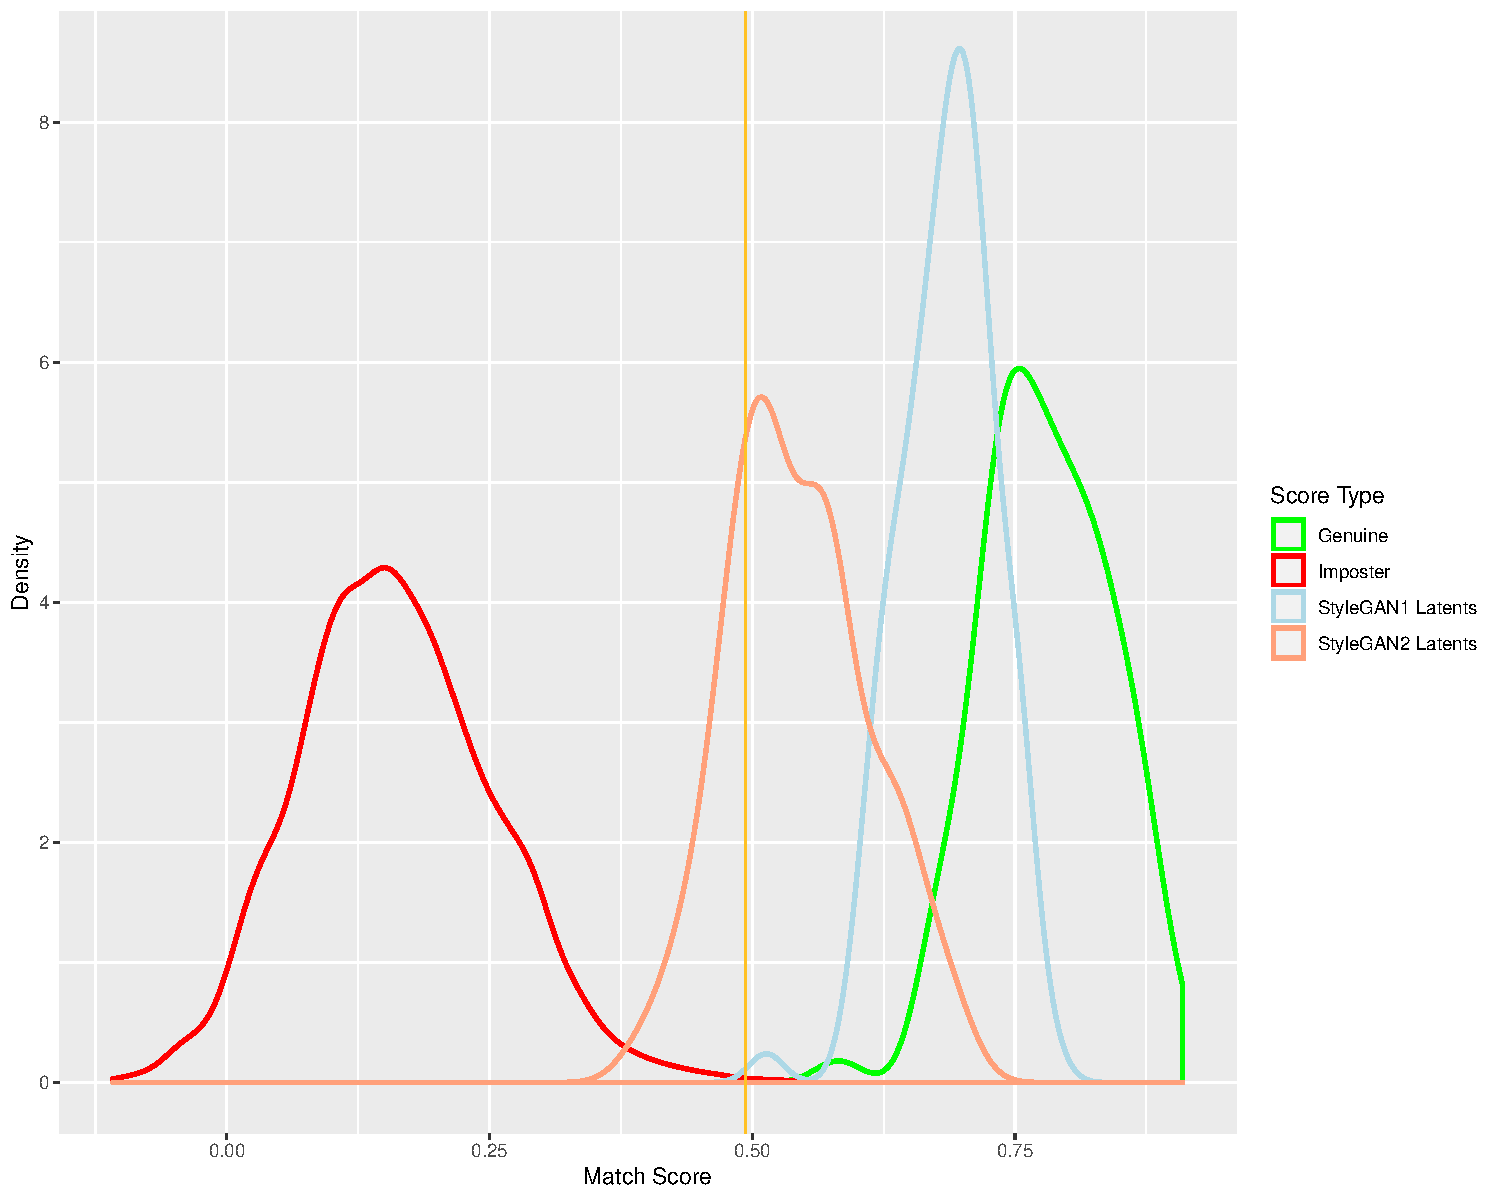
\includegraphics[width=0.8\linewidth]{dlib_fr_latent_hist.pdf}
    \caption{Plot of the latent score distributions for each GAN-based method. The genuine and impostor distributions are the same as before. This plot shows that the images generated from latent representations without morphing already suffer from inaccuracies.}
    \label{latent_plot}
\end{figure}
\section{Discussion}
% GAN generated morphs take too long and aren't good enough according to these results
\par
From our evaluation, it seems that the stylegan-encoder and the StyleGAN2 projector are not feasible for generating high quality morphs yet. In order for a method to successfully trick a face recognition algorithm, the match score of the morph must be greater than the threshold the algorithm uses. For dlib-based algorithm and the common threshold of 0.1\% FMR, the algorithm will only be fooled 19.2\% of the time by the StyleGAN based method. For the StyleGAN2 based method, this is even worse at about 6\%. This contrasts with the landmark-based morphs (at 58\%) which are already unreliable for consistently generating successful morphs.
% Talk about how the latent encoding isn't good enough
\par
The cause of the low scores likely comes from the latent learning process. Figure \ref{latent_plot} shows the match score distributions for the images generated directly from the latent vectors before any morphing takes place. Since no morphing occurs at this stage, each latent image should represent the same face and ideally look exactly like the input images used to learn it. However, the scores tend to be lower for the stylegan-encoder latents and much lower for the StyleGAN2 projector latents (only 76.5\% of the StyleGAN2 latents surpass the threshold). Even though the stylegan-encoder latents all surpass the threshold like the genuine distribution, having lower match scores (median of 0.690 vs. 0.776 for genuines) means that there are slight inaccuracies which will propagate into the morphs.
% Talk about difference between StyleGAN1 and StyleGAN2 latent (refer to background information)
\par
It is quite interesting that the StyleGAN2 morphs and latents perform much worse than their stylegan-encoder counterparts even though StyleGAN2 is supposed to be of higher quality. This is likely due to the design of the StyleGAN2 projector. Recall that NVIDIA wanted the projector to focus on finding representations that the generator itself would have produced, whereas the stylegan-encoder extends the latent space to allow for encoding of arbitrary images. As a result, the images generated by the stylegan-encoder latents are usually much closer to the original image compared to the StyleGAN2 projector \cite{stylegan2}.
% Talk about how you could get better results by morphing already similar faces
\par
However, the latent representation is not the only problem. Conceptually, the morphing alone would already decrease match scores since we are trying to find a morph image that is somewhere in between two different faces. It is unclear whether it is possible to find a single face that would look exactly like two different distinct faces or what the upper bound on the similarity can be. Nonetheless, we can generate higher scoring morphs if the input faces for the morph are already similar. The more similar the inputs are, the higher our morph scores will be since there's less of a transition between the two.
% Talk about GANs not having landmark artifacts but have their own


\section{Related Work}
\par
Abdal \textit{et al.} \cite{abdal2019image2stylegan} was one of the first to explore latent embedding interpolation as a method for morphing iamges using GANs. Their work primarily focused on gaining valuable insight into the structure of the StyleGAN latent space, leading to an efficient algorithm for generating latent embeddings (Image2StyleGAN) and an evaluation of how meaningful the embeddings are. Similarly to the stylegan-encoder, they generate latent space embeddings by optimizing the latent vector to minimize the loss between the given image and the image generated from this latent vector.
\par
Building on their previous work, Abdal \textit{et al.} recently developed Image2StyleGAN++ \cite{abdal2020image2stylegan} which improves quality by preserving high frequency features and adds capabilities for local image editing of the embedded images. The embedding generated images which they show in their paper impressively capture minute details from the original given image. If such an embedding process can achieve high match scores for the latent images, then their algorithm may lead to great advancements for GAN generated morphs.
% \cite{venkatesh2020gan}
\par
\cite{venkatesh2020gan} performed a similar evaluation of StyleGAN's morphing abilities as we did. However, 
% \cite{zhang2021mipgan}
% \cite{sarkar2020vulnerability}


\section{Future Work}
% StyleGAN2-Ada (seems to take about 10 min for projecting)
% Test with commercial face recognition algorithms
% Perhaps build an encoder for StyleGAN2 that doesn't have the restrictions of the projector
% Generate morphs of similar looking faces and see how good their scores are in comparison

\section{Conclusion}

\bibliographystyle{unsrt}
\bibliography{paper}

\end{document}
